% В этом шаблоне используется класс spbau-diploma. Его можно найти и, если требуется, 
% поправить в файле spbau-diploma.cls
\documentclass{spbau-diploma}
\usepackage{wasysym}
\usepackage{subfiles}
\usepackage{enumitem}
\usepackage{graphicx}
\usepackage{svg}
\usepackage{tabularx}
\usepackage{caption}
\usepackage{subcaption}
% \usepackage{incgraph,tikz}
% \usepackage{chngcntr}
% \counterwithin{figure}{section}
% \counterwithin{table}{section}
% \counterwithin{equation}{section}
% \captionsetup[table]{justification=raggedleft,singlelinecheck=off}

\def\bbljan{January}  \def\bblfeb{February}  \def\bblmar{March}
\def\bblapr{April}    \def\bblmay{May}       \def\bbljun{June}
\def\bbljul{July}     \def\bblaug{August}    \def\bblsep{September}
\def\bbloct{October}  \def\bblnov{November}  \def\bbldec{December}

\begin{document}
% \begin{titlepage}
% \incgraph[documentpaper][width=\paperwidth,height=\paperheight]{images/TitlePage.pdf}
% \end{titlepage}


\includepdf[pages=-]{images/TitlePage.pdf}
\maketitle
\setcounter{page}{2}
% \pagebreak
% \my@body14pt
\newgeometry{a4paper,top=20mm,bottom=20mm,left=30mm,right=15mm,nohead,includeheadfoot}
\tableofcontents

\section*{Введение}\label{sec:introduction}

\subsection*{Актуальность и релевантные работы}
Задача определения авторства возникает в разных областях на протяжении многих лет. Работы неизвестных или пожелавших остаться анонимными авторов существуют в литературе, живописи, музыке, и программирование не является исключением. Необходимость определить разработчика, стоящего за кодом, возникает при поиске авторов вредоносного программного обеспечения, решении вопросов интеллектуальной собственности.

Подходы к решению задачи определения авторства основываются на предположении, что каждый автор обладает уникальный стилем, точно так же как уникальным почерком или отпечатком пальца. Идея определения набора характеристик или метрик кода, которые отражают стиль его автора, интересует исследователей не менее трех десятилетий \cite{Halstead1972,Oman1989}. Статистический анализ стилистики кода, текстов или живописи называется стилометрией. Он основывается на подсчете метрик или факторов по исследуемому материалу и дальнейшем анализе полученных численных представлений.

Предыдущие исследования в области определения авторства кода были мотивированы проверкой авторства \cite{Elenbogen2008,Kothari2007}, поиском плагиата \cite{Ottenstein1976,Liu2006}, определением авторов вредоносных программ \cite{Layton2010,Caliskan2015}. Для использования автоматических методов во всех перечисленных задачах требуется хорошее тестирование. Для этого необходим набор данных, на котором оно будет производиться. В существующих работах в качестве датасетов применялись студенческие домашние задания \cite{Frantzeskou2007,Elenbogen2008,Krsul1997}, примеры кода из книг \cite{Oman1989,Frantzeskou2006}, задачи соревнований по программированию \cite{Rosenblum2011,Caliskan2015,Alsulami2017,Simko2018} и проекты с открытым исходным, написанные одним автором \cite{Shevertalov2009,Kothari2007,Yang2017,Zhang2017}. У всех перечисленных типов датасетов есть свои недостатки: они отличаются от промышленного кода и у них есть ограничение на количество примеров, доступных для каждого автора.

В предыдущих работах не изучалось масштабирование решений на случай, когда для каждого автора доступны не десятки или сотни примеров, а десятки тысяч. Это связано с ограничениями имеющихся датасетов: такие объемы доступны только в крупных промышленных проектах, а в них одновременно работает большое количество программистов и сложно разделить код между ними, чтобы собрать примеры, для которых автор известен. Помимо этого, лучшие модели на данный момент для определения авторства по коду на языках C++ и Java используют факторы, специфичные для конкретных языков, что усложняет использование предложенных методов для других языков.

\subsection*{Цель и задачи}
Данная работа ставит целью создание универсального относительно языка решения, которое улучшает или повторяет существующие результаты в определении авторства для C++, Java и Python, проверка его масштабируемости на разные объемы данных, доступных для каждого автора, сравнение с имеющимися исследованиями. Для этого ставятся следующие задачи:
\begin{itemize}
    \item Научиться собирать данные для обучения и тестирования моделей, определяющих авторство кода, из проектов с произвольным количеством авторов.
    \item Создать набор датасетов для анализа применимости моделей в разных условиях: при разном количестве данных, несбалансированном количестве примеров, доступном для каждого автора, разделяя примеры в обучающей и тестовой выборке по времени.
    \item Создать модель, позволяющую работать одинаковым образом с кодом на различных языках и адаптировать её для работы с произвольным объемом доступных данных.
    \item Протестировать модель на собранных датасетах и сравнить с существующими решениями, используя данные, на которых они тестировались.
\end{itemize}

\subsection*{Достигнутые результаты}
В рамках данной работы был реализован инструмент для сбора данных из проектов с произвольным числом автором, которые разрабатывались с использованием системы контроля версия (VCS, version control system) git. Для этого история проекта разбивается на отдельные изменения, для каждого из которых известен автор. Эти изменения в свою очередь разбиваются на изменения методов или классов, которые и составляют итоговый датасет. Такой подход снимает ограничения, которые были у предыдущих наборов данных: есть возможность использовать промышленный код, нет ограничения в выборе проектов и количестве доступных примеров.

При помощи инструмента были собраны данные обо всех изменениях методов в IntelliJ IDEA\footnote{\url{https://github.com/jetbrains/intellij-community}}, втором по размеру проекте на GitHub с открытым исходным кодом на языке Java. Это 700 тысяч созданных методов и 2 миллиона изменений, принадлежащих 500 разработчикам. Из них было составлено 5 датасетов, предназначенных для тестирования моделей в разных условиях (подробнее в главе 3).

Было реализовано две модели: для работы в условиях небольшого количества примеров (от нескольких до сотен), доступных для каждого разработчика и в условиях большого (десятки и сотни тысяч). Обе модели основываются на технике представления кода при помощи контекстов в абстрактном синтаксическом дереве (AST, abstract syntax tree) \cite{Alon2018}. Использование AST для определения авторства по коду уже позволяло улучшать результаты в нескольких недавних работах \cite{Caliskan2015,Alsulami2017}.

Полученные модели были протестированы на наборах данных для C++, Java и Python, результаты тестирования на которых приводили исследователи в недавних работах. Полученная точность в случае Python и Java оказалась лучше, чем у предыдущих решений и повторила предыдущие результаты в случае C++ (подробнее в главе 6). Для датасетов, собранных на основе IntelliJ IDEA, результаты не сравниваются с предыдущими решениями из-за отсутствия их реализации в открытом доступе или того, что имеющиеся реализации не поддерживают Java.

\subsection*{Структура работы}
В главе 1 представлен обзор предыдущих исследований в области, история развития подходов к определению авторства с точки зрения данных, факторов и методов машинного обучения. 

В главе 2 представлена предложенная техника сбора данных из проектов с произвольным числом авторов, реализованный инструмент для сбора данных и собранные датасеты.

В главе 3 приводятся технические детали и архитектура созданных моделей.

В главе 4 представлены численные результаты проделанной работы, результаты проведенных экспериментов и приведено исследование поведения моделей в разных условиях.

В последней главе анализируется проделанная работа и приводятся возможные перспективы дальнейшей деятельности.
\section{Обзор литературы}\label{sec:literature}

\subsection{История развития области}

Первоначально задача установления авторства появилась в литературе не позднее, чем в XIX веке. Первые исследования, связанные с авторством программного кода, появились только в 1970-е \cite{Ottenstein1976} и основывались на теории программного обеспечения, разработанной Холстедом \cite{Halstead1972,Halstead1975}. Теория утверждала, что всего четырёх метрик и их комбинаций достаточно, чтобы передать внутренние свойства программы, в том числе, различия в коде, написанном разными авторами. Метрики, названные метриками Холстеда, приведены в таблице \ref{tab:halstead}.

В дальнейшем было показано, что предсказания теории расходятся с эмпирическими данными \cite{Hamer1982,Shen1983}, но, несмотря на это, она дала начало исследованиям по поиску сходств в программах. Первоначально они были направлены на автоматическое определение списывания в домашних заданиях.

В дальнейшем теорию активно развивали: был предложен алгоритм для быстрого вычисления метрик по коду \cite{Bulut1974}, показана связь между размером проекта, временем, потраченным на его разработку и метриками Холстеда \cite{Albrecht1983}. Фитцсиммонс \cite{Fitzsimmons1978} продемонстрировала, что при достаточно большом количестве программ теория программного обеспечения даёт точные оценки на число ошибок, допущенных в коде. Несмотря на поддержку теории частью учёных, подвергались критике её расхождения с эмпирическими данными \cite{Hamer1982, Shen1983}.

\vskip 1em
	\begin{table}[ht]
        \caption{Метрики Холстеда \cite{Halstead1972}.}
		\centering
        \begin{tabular}{|c|c|}
            \hline
            \textbf{Метрика} & \textbf{Определение} \\ \hline
            n1 & Число различных операторов \\ \hline
            n2 & Число различных операндов \\ \hline
            N1 & Суммарное число операторов \\ \hline
            N1 & Суммарное число операндов \\ \hline
            \end{tabular}
		\label{tab:halstead}
   \end{table}

Задача определения авторства исходного кода впервые привлекла внимание исследователей в 1989 году. Оман и Кук \cite{Oman1989} показали, что авторов программ можно различить с хорошей точностью, основываясь на статистическом анализе метрик форматирования. К ним относится расстановка переносов строк, отступов, длины названий переменных и функций, типы комментариев. Авторы не учитывали, что часть из этих метрик легко изменить при помощи текстовых редакторов или сред разработки.

Затем, Спэффорд и др. \cite{Spafford1993} впервые заговорили о применении автоматического определения авторства кода для решения вопросов интеллектуальной собственности. Авторы утверждали, что у каждого программиста есть свой уникальный стиль, по которому его можно определить, точно так же, как это делается по почерку в судебно-медицинской экспертизе. Несмотря на отсутствие эмпирической проверки этих утверждений, в работе было приведено большое количество метрик или факторов, по которым можно определять стиль программиста: использование библиотек, возможностей языка, допускаемые ошибки, стиль форматирования и комментариев, названия переменных и ошибки в них. В дальнейшем они использовались во многих работах по установлению авторства \cite{Macdonell1999,Ding2004,Lange2007,Kothari2007,Caliskan2015,Yang2017}.

Определение авторства в литературе и программировании являются похожими по формулировке задачами, но между областями есть существенные различия. В работе \cite{Krsul1997} авторы пришли к выводу, что определить автора фрагмента кода сложнее, чем литературного текста. Это вызвано тем, что разработчики переиспользуют код, работают в командах, используют среды разработки, автоматически форматирующие код, используют сторонние библиотеки и инструменты. В работе \cite{Sallis1996} было показано, что несмотря на вышеописанные различия, методы из области обработки естественного языка (ОЕЯ или NLP, Natural Language Processing) могут давать хорошие результаты, если будут использованы вместе с метриками программного обеспечения.

Последующие работы \cite{Krsul1997, Gray1998, Macdonell1999} сфокусировались на расширении множества используемых факторов, в том числе добавляя факторы, применимые для конкретного языка программирования, например, число директив препроцессора в C++ \cite{Macdonell1999}. В 2004 году Динг и др. \cite{Ding2004} применили отбор факторов для определения авторства кода на Java. Они использовали набор метрик из предыдущих работ и отфильтровали его при помощи пошагового дискриминантного анализа и дисперсионного анализа. Оба способа показали улучшение точности с 62\% до 85\% по сравнению с использованием всех метрик.

В то время как вышеописанные исследования работали с метриками, которые понятны человеку и на основе которых люди могут считать код похожим, в работе Франческу и др. \cite{Frantzeskou2006, Frantzeskou2007} были использованы N-граммы, полученные по коду. N-граммы — это последовательности из N идущих подряд символов, например, 4-граммы строки “СТРОКА” это {“СТРО”, “ТРОК”, “РОКА”}. Авторы построили профиль для каждого автора, состоящий из нескольких тысяч наиболее часто встречающихся N-грамм в его документах. Определение автора нового документа состояло из построения по нему набора N-грамм такого же размера и нахождения самого близкого профиля по размеру пересечения с набором. Такой подход показал высокую точность при различении как студенческих заданий на Java, так и проектов с открытым исходным кодом, при этом будучи простым с точки зрения вычислений и независимым от языка программирования.

Из-за простоты и эффективности анализа N-грамм он использовался во многих последующих работах \cite{Burrows2007, Krishna2006, Layton2010}. Бёрроуз и др. \cite{Burrows2007} исследовали применение N-грамм к изменённой версии кода, в которой оставлены только операторы и ключевые слова. Кришна и др. \cite{Krishna2006} использовали подход для поиска компьютерных вирусов. Лейтон и др. \cite{Layton2010} определяли с его помощью авторов фишинговых программ.

Общей проблемой анализа N-грамм для определения авторства является выбор N. В разных работах, в зависимости от данных и метрики оценки, оптимальные значения варьируются от 4 \cite{Kothari2007} до 20 \cite{Burrows2007}. Второй проблемой оказалось падение точности при увеличении числа различаемых программистов \cite{Burrows2007}. Последующие работы переключились с анализа синтаксического сходства кода на анализ его семантики \cite{Vinod2012, Caliskan2015, Chen2010}.


К 2007 году сформировался общий подход к решению задачи определения авторства, подробно описанный в работе Котари \cite{Kothari2007}. Он имеет следующую структуру: сперва собирается набор фрагментов кода, для которых известны авторы. Фрагментами могут быть как целые файлы, так и отдельные классы или методы. Собранный набор данных разделяется на обучающую или тренировочную и тестовую выборки. По каждому фрагменту в обучающей выборке считается заданный набор метрик (например, частоты N-грамм \cite{Frantzeskou2006} или метрики, специфичные для языка \cite{Macdonell1999}), называемый численным представлением фрагмента. Затем выбирается модель для решения задачи и обучается на тренировочных представлениях. Она может агрегировать информацию для отдельных авторов в профили или же пользоваться ей в явном виде. Качество обученной модели проверяется на тестовой выборке.

\subsection{Выбор данных}

Получаемые результаты зависят от того, какие данные были собраны. Чтобы можно было утверждать о применимости модели на практике, она должна быть протестирована на данных, близких к реальным. В исследованиях 90-х годов \cite{Krsul1997, Leach1995} в качестве датасетов использовались домашние задания студентов. Это вызывало проблемы с распространением данных, поскольку их требовалось анонимизировать, удалять комментарии.

Помимо домашних заданий в работах использовались примеры кода из книг по программированию и код, представленный в качестве примера авторами компиляторов \cite{Macdonell1999, Oman1989}. В случае таких фрагментов считалось, что весь код в одной книге или одном компиляторе написан одним человеком, что не обязательно является правдой.

С ростом популярности программ с открытым исходным кодом и сервисов для их загрузки исследователи стали использовать их в качестве датасетов. Так, использовались фрагменты кода, скачанные на freshmeat\footnote{\url{http://freshmeat.sourceforge.net/}} \cite{Frantzeskou2006}, SourceForge\footnote{\url{http://sourceforge.net/}} \cite{Lange2007, Shevertalov2009}, planet-source-code\footnote{\url{https://www.planet-source-code.com/}} \cite{Bandara2013}. Такие данные ближе к промышленному коду, чем домашние задания или код из книг, но при этом фрагменты разных авторов могут относиться к проектам разной тематики. Это вызывает у исследователей опасение, что итоговое решение учится различать тематику проекта, а не его автора \cite{Caliskan2015}.

Розенблум и др. \cite{Rosenblum2011} стали первыми, кто в качестве датасета использовались решения участников Google Code Jam (GCJ). GCJ — ежегодное соревнование по программированию, проводимое компанией Google с 2008 года. Соревнование состоит из нескольких раундов, в каждом из которых участникам предлагается набор из нескольких алгоритмических задач, которые требуется решить за ограниченное время. Хотя решения принимается на большинстве популярных языков программирования, чаще всего используются C++, C и Python. Все корректные решения, отправленные во время соревнования, доступны для скачивания и активно используются исследователями, занимающимися задачей определения авторства \cite{Rosenblum2011, Caliskan2015, Alsulami2017, Simko2018}. Это вызвано тем, что все участники решают одни и те же задачи, а значит их код должен выполнять одну функцию, различаясь только индивидуальными особенностями авторов. Тем не менее, использование данных GCJ подвергается критике \cite{Dauber2017} за свою искусственность: код в решениях алгоритмических задач может сильно отличаться от промышленного кода.

Помимо нового подхода к выбору данных, в работах Розенблума и др. \cite{Rosenblum2010,Rosenblum2011,Rosenblum2011-2} был предложен новый способ определения автора по бинарным файлам и возможность восстановить набор инструментов, которым бинарный файл был получен: компилятор, его версию и уровень оптимизации. В этой серии работ была предложена методика получению факторов по бинарному коду. Для этого сперва из бинарного файла извлекается код отдельных функций или логических блоков и граф потока управления. Затем в коде ищутся идиомы — последовательности из 1-3 инструкций, содержащие низкоуровневую информацию о логике кода — наличие которых является фактором. В графе потока управления ищутся графлеты — подграфы из 3 вершин, которые отражают локальную структуру программы.  Количества найденных графлетов каждого типа является фактором. В итоге авторы получили точность 51\% при определении автора бинарного файла, выбирая из 191 автора.

\subsection{Выбор методов}

Помимо развития в выборе данных и метрик происходило развитие в выборе методов. Для определения авторства исходного кода применялись разные методы машинного обучения.

Часть работ использовали подходы, основывающиеся на поиске похожих фрагментов: метод ближайших соседей \cite{Keselj2003, Lange2007, Frantzeskou2006}, ранжирование \cite{Burrows2007, Shevertalov2009}. Суть этих подходов заключается в подсчёте расстояния между численными представлениями кода. Автором фрагмента кода считается автор большинства близких к нему фрагментов обучающей выборке. Расстоянием может выступать расстояние в векторном пространстве \cite{Shevertalov2009}, пересечение гистограмм \cite{Lange2007} или специально подобранная метрика, например, пересечение наборов N-грамм \cite{Frantzeskou2006,Frantzeskou2007}. В работе Бёрроуза и др. \cite{Burrows2007}, исследовавшей определение авторства на основе ранжирования, сравнивалась эффективность четырёх расстояний: косинусной меры, языковой модели со сглаживанием Дирихле, BM25 и предложенной авторами метрики. Лучшие результаты показало использование BM25, что согласуется с результатами в области информационного поиска \cite{Robertson2009}.

Также исследователи применяли вероятностные методы: байесовский классификатор \cite{Kothari2007} и логистическую регрессию \cite{Bandara2013}. Суть этих методов заключается в оценке вероятности того, что фрагмент кода принадлежит автору, при условии того, что в нём встречаются определённые N-граммы символов или токенов. Несмотря на хорошие результаты обеих работ относительно других исследований своего времени, в случае вероятностных подходов сложнее расширять множество факторов, поэтому их используют реже в пользу других методов.

В недавних работах популярностью пользуются методы, работающие с набором факторов как с векторами. К таким методам относится дискриминантный анализ \cite{Ding2004, Hayes2008, Hayes2010} и метод опорных векторов \cite{Rosenblum2011, Wisse2015, Meng2016}. Сперва по фрагментам кода подсчитывается набор из $n$ метрик, образуя $n$-мерный вектор численного представления фрагмента. Примеры кода разных авторов образуют множества из векторов в $n$-мерном пространстве, и, если подобран качественный набор метрик, множества можно различить. Дальнейшую задачу дискриминантный анализ и метод опорных векторов решают по-разному. 

Дискриминантный анализ трактует векторы фрагментов кода как примеры, полученные из разных случайных распределений. Задача определения авторства в таком случае сводится к подбору параметров распределений, которые наилучшим образом объясняют примеры из обучающей выборки, а для примеров из тестовой выборки в качестве предсказания берется автор, к распределению которого вектор кода относится с наибольшей вероятностью.

Метод опорных векторов основан на поиске поверхности, которая наилучшим образом отделяет в пространстве векторы одного класса от всех остальных. В самом простом случае поверхностью является плоскость, в более сложных применяется метод опорных векторов с ядром, что позволяет искать более сложные поверхности. Для применения метода к новым примерам вычисляется их положение относительно разделяющих поверхностей.

Ещё одним методом, использовавшимся для решения задачи определения авторства, является решающее дерево. Оно применялось в работе Эленбогена и др. \cite{Elenbogen2008}. Для построения дерева авторы применяли алгоритм C4.5 \cite{Quinlan1993}. Это жадный алгоритм, который строит дерево от корня к листьям, в каждой вершине выбирая фактор и его значение такое, что оно наилучшим образом разбивает часть выборки, дошедшую до вершины, на две части. Затем, алгоритм рекурсивно применяется в двух новых вершинах. Когда дерево построено, чтобы уменьшить переобучение, в нём обрезается часть веток.

Идею решающего дерева развивает случайный лес. Вместо построения одного решающего дерева, используя все доступные данные и факторы, строится от нескольких до сотен или даже тысяч деревьев. Каждое из них строится по случайной части обучающей выборки, используя случайный поднабор факторов.  При определении ответа каждое полученное дерево принимает решение и решение большинства принимается за ответ.  Случайный лес использовали в нескольких недавних работах по установлению авторства \cite{Caliskan2015} и имитации стиля \cite{Simko2018}.

В исследовании по определению авторства Калискан и др. \cite{Caliskan2015} продолжили работу с данными GCJ. В то время как большинство предыдущих исследований работали с кодом как с обычным текстом, отличающимся только форматированием и наличием специальных слов, они использовали факторы, полученные по абстрактному синтаксическому дереву (AST, Abstract Syntax Tree), соответствующему коду. Такие факторы называют синтаксическими, к ним в данной работе относились частоты встречаемости и средние глубины отдельных вершин разных типов и их пар, соединённых ребром. Использование AST позволяет передать внутреннюю структуру кода, которая в свою очередь отвечает за его функциональность. Помимо синтаксических также в работе применялся большой набор метрик форматирования и лексических, что породило около 100 тысяч факторов. Их количество затем было сокращено до 1000 наиболее полезных, при этом критерием отбора была совместная информация между значением фактора и автором. Описанный набор метрик затем использовался другими исследователями \cite{Yang2017}.

По полученному после подсчёта и фильтрации факторов численному представлению Калискан и др. обучили случайный лес из 300 деревьев. В результате они получили решение, которое хорошо масштабировалось на данных GCJ: 98\% точности при различении кода 250 авторов на C++, 92\% при различении 1600. Стоит отметить, что работ со сравнением такого количества программистов ранее не проводилось и результат остаётся лучшим для данных GCJ  на языке C++. Препятствием к дальнейшему увеличению масштаба стали ограничения датасета: только у 1600 участников было 9 решений по одним и тем же задачам.

С развитием методов, использующих нейронные сети в работе с изображениями \cite{He2016}, обработке естественного языка \cite{Young2018} и распознавании речи \cite{Zhang2018-speech}, сети стали применяться и в определении авторства. Нейронная сеть или нейросеть это математическая модель, построенная по принципу организации нейронов в мозгу человека. Нейросеть состоит из элементов, соединенных направленными связями, по которым данные передаются от входных нейронов к следующим элементам, вплоть до выходных нейронов. Элементы применяют к полученным на вход данным различные математические операции: линейную комбинацию, применение нелинейной функции, свертку, сдвиг и так далее. Набор элементов и связей между ними описывается архитектурой нейросети. В области обработки естественного языка для решения задач активно применяются рекуррентные нейронные сети \cite{Jordan1990} и, в частности, LSTM \cite{Hochreiter1997}.

Идея работы с AST при помощи нейронных сетей была продолжена Алсулами и др. \cite{Alsulami2017}. Вместо дальнейшего расширения набора факторов, они применили модификацию LSTM для работы с деревьями \cite{Tai2015}. Она работает следующим образом: каждому типу вершины в AST и токену сопоставляется вектор, называющийся эмбеддинг, изначально случайный, но изменяющийся в процессе обучения сети. Дерево обходится в глубину, в листьях сеть получает на вход эмбеддинг токена, относящегося к листу, в остальных вершинах — векторы, полученные в детях, и эмбеддинг типа текущей вершины. В результате в корне дерева сеть генерирует вектор, являющийся представлением всего дерева. По нему ещё одним линейным слоем с функцией активации softmax делается предсказание. Сеть обучается при помощи стохастического градиентного спуска и алгоритма обратного распространения ошибки.

Тестирование проводилось для языков Python и C++. Для Python были использованы решения по 10 задачам 70 участников GCJ. Для C++ использовались проекты 10 авторов, размещённые на GitHub. Модель достигла точности 88.8\% при распознавании кода на Python 70 авторов, что является лучшим из известных результатов на данный момент.

В работах по установлению авторства кода использовали не только разные архитектуры сетей, но и методы оптимизации для их обучения. В 2017 году Янг и др. \cite{Yang2017} применили набор факторов из работы Калискан и др. \cite{Caliskan2015}, объединив некоторые из них в более общие, и обучили трёхслойную нейросеть для определения автора по ним. Они сравнили два метода обучения: стохастический градиентный спуск (SGD, stochastic gradient decent) и метод роя частиц (PSO, particle swarm optimisation) \cite{Kennedy1995}. Сравнение производилось на датасете из 40 проектов на Java, каждый из которых был написан одним автором. Результаты при использовании PSO оказались значительно лучше, чем при стохастическом градиентном спуске, который обычно используется при обучении нейросетей: 91\% против 76\%. Результат является наилучшим на данный момент для этого набора данных.

Изменение методов машинного обучения, использовавшихся для решения задачи определения авторства, происходило одновременно с эволюцией методов для решения других задач в области машинного обучения на исходном коде. К ним относится генерация кода, определение тематики, генерация описания по фрагменту кода, определение имени метода.

Недавний прогресс в определении имени метода и генерации описания кода связан с техникой векторного представления кода, предложенной Алоном и др. в 2018 году \cite{Alon2018, Alon2019}. Её можно рассматривать как обобщение использования биграмм типов вершин в AST и токенов, предложенных в работе Калискан и др. \cite{Caliskan2015}. По фрагменту кода строится AST и из него извлекаются тройки из пути между парой листьев и токенов, соответствующим им. Такие тройки называются контекстами. Фрагмент представляется набором контекстов, ему соответствующим. Контексту сопоставляется вектор, состоящий из конкатенации эмбеддингов токенов и пути. Затем векторы контекстов агрегируются при помощи механизма внимания \cite{attention}. Это механизм, позволивший улучшить результаты в задачах обработки естественного языка \cite{Young2018}. Вектором для фрагмента является взвешенная сумма векторов контекстов, где весами являются значения внимания.

\subsection{Выводы}

\begin{itemize}
    \item Для трёх разных языков, Java, C++ и Python, наилучшие результаты показывают разные работы. Решения для Java \cite{Yang2017} и C++ \cite{Caliskan2015} используют факторы, специфичные для конкретного языка, что затрудняет их адаптацию к другим. Решение для Python \cite{Alsulami2017} использует только AST, поэтому является универсальным, при этом показывая очень высокую точность. Это позволяет надеяться на то, что используя AST можно получить универсальное решение, показывающее хорошие результаты сразу для нескольких языков.
    \item В исследованиях не рассматривалась работа с большим количеством данных для каждого автора. Это актуально в задачах проверки авторства, кластеризации и профилировании разработчиков. Ограничением для подобных исследований является отсутствие датасета соответствующего размера.
    \item Датасеты в недавних работах состоят из задач олимпиадного программирования \cite{Rosenblum2011,Caliskan2015,Alsulami2017,Simko2018} или из проектов с одним автором \cite{Zhang2017,Alsulami2017,Wisse2015,Bandara2013,Yang2017}. Решения задач на соревнованиях значительно отличаются от промышленного кода: участникам требуется написать решение максимально быстро, что может быть сделано в ущерб читаемости и архитектуре. Чаще всего решение состоит из одного файла, где большая часть кода находится в одной функции. В дополнение к отличиям от промышленного кода, количество доступных данных значительно отличается от обычных проектов, поскольку программисты гораздо реже участвуют в соревнованиях, чем пишут код на работе. В датасетах из проектов, написанных разными людьми, присутствует разница в предметной области между кодом разных авторов. Решение, которое показывает высокую точность на подобных датасетах, может показывать другие результаты применительно к коду разных авторов в одной предметной области, что важно для поиска авторов вредоносных программ. Проблемы обоих видов датасетов можно решить, если собирать данные из крупных проектов с большим количеством авторов.
\end{itemize}
\section{Данные}\label{sec:data}
Чтобы обучить модель машинного обучения и протестировать её качество, нужен датасет. У имеющихся датасетов есть слабые стороны, которые указывались в работах других исследователей. В этой главе предлагается новый подход к сбору данных для оценки качества решений задачи определения авторства, описывается реализованный инструмент для создания датасетов, использующий этот подход и датасеты, собранные с его помощью.

\subsection{Ограничения существующих датасетов}
Прошлые исследования в области определения авторства исходного кода работали с наборами данных нескольких видов: домашние задания студентов \cite{Frantzeskou2007,Elenbogen2008,Krsul1997}, примеры кода в книгах по программированию \cite{Oman1989,Frantzeskou2006}, решения задач соревнований по программированию \cite{Rosenblum2011,Caliskan2015,Alsulami2017,Simko2018}, проекты с открытым исходным кодом, имеющие одного автора \cite{Shevertalov2009,Kothari2007,Yang2017,Zhang2017}. Первые три типа данных значительно отличаются от промышленного кода: студенты имеют меньше опыта, чем профессиональные разработчики, примеры в книгах – это короткие и неполные фрагменты, на соревнованиях участникам важно написать программу быстро, не задумываясь о читаемости и качестве написанного. Отличия не позволяют однозначно утверждать, что решение, демонстрирующее хорошую точность на таких датасетах, будет так же хорошо работать для промышленного кода, что важно при его применении для решения вопросов интеллектуальной собственности.

Существующие исследования работают не с произвольными проектами с открытым исходным кодом, а только с имеющими одного автора или такими, где хотя бы 90\% кода принадлежит одному разработчику. В датасетах, состоящих из таких проектов, код разных авторов соответствует разным проектам, а значит может иметь разную тематику и функциональность. Из-за этого нельзя быть уверенными в том, что полученное решение будет хорошо работать, если будет применяться для различения кода разработчиков, работающих в одной области или реализующих схожую функциональность, хотя это важно при поиске авторов вредоносного ПО, поиске плагиата, проверке авторства.

Также, у всех четырёх типов данных есть ограничение на количество фрагментов кода, доступных для каждого автора: ограниченный набор задач на соревнованиях и в домашних работах, требуемое количество поясняющих примеров в книгах. Проекты с одним автором также редко состоят из более чем нескольких сотен файлов, поскольку при дальнейшем росте проекта у него появляются пользователи, которые начинают самостоятельно предлагать изменения и вносить свой вклад в его развитие. В то же время, профессиональные программисты пишут гораздо большие объемы кода. Например, в проекте IntelliJ IDEA есть 40 разработчиков, каждый из которых добавил не менее 10000 методов.

\subsection{Методика сбора данных}
В этой работе предлагается метод сбора данных из проектов с произвольным числом разработчиков, разрабатываемых с использованием системы контроля версий (VCS, version control system). Необходимость в VCS не является сильным ограничением, поскольку в настоящее время это общепринятая практика. Самой популярной платформой для загрузки программ с открытым кодом является GitHub\footnote{\url{https://github.com/}}, поддерживающая VCS git. По состоянию на конец 2018 года, платформой пользуется более 30 миллионов разработчиков, создавших 96 миллионов репозиториев \cite{GithubStats}. Датасеты, состоящие из проектов на GitHub, уже использовались в работах по определению авторства \cite{Wisse2015,Yang2017,Alsulami2017,Zhang2017}.

В проектах, использующих VCS, изменения добавляются группами, которые называются коммитами. Коммит чаще всего принадлежит одному автору и состоит из набора изменений, которые могут затрагивать произвольное число файлов. В таблице \ref{tab:repositories} приведены 10 репозиториев на GitHub с самым большим числом коммитов. Каждый коммит можно разбить на изменения, затрагивающие части кода определенного уровня: изменения методов, классов, файлов. Из таких изменений в свою очередь можно составить датасет, поскольку для каждого из них автор известен благодаря VCS. В этой работе рассматриваются изменения отдельных методов.

\vskip 1em
	\begin{table}[ht]
		\caption{Репозитории на GitHub с самым большим числом коммитов}
		\centering
    	\begin{tabular}{| l | l | l |}
    		\hline
    		\textbf{Репозиторий}  & \textbf{Коммиты (тыс.)} & \textbf{Основной язык} \\ \hline
    		torvalds/linux & 782 & C \\ \hline
    		LibreOffice/core & 428 & C++ \\ \hline
    		liferay/liferay-portal & 283 & Java \\ \hline
    		jsonn/pkgsrc & 266 & Makefile \\ \hline
    		freebsd/freebsd & 254 & C \\ \hline
    		JetBrains/intellij-community & 230 & Java \\ \hline
    		cms-sw/cmssw & 194 & C++ \\ \hline
    		openbsd/src & 192 & C \\ \hline
    		NixOS/nixpkgs & 154 & Nix \\ \hline
    		Wikia/app & 152 & PHP \\ \hline
    	\end{tabular}
		\label{tab:repositories}
	\end{table}

Использование такого подхода затруднено тем, что git, являющийся самой популярной VCS, не хранит подробную информацию об изменениях. Это означает, что чтобы получить информацию об изменении метода, нужно найти его в старой и новой версии файла, что может быть проблематичным в случае переименования или изменения сигнатуры. Для решения этой проблемы была использована библиотека GumTree \cite{GumTree}, позволяющая строить AST по коду на языке Java и искать по версиям файла до и после коммита изменившиеся методы и соответствующие им поддеревья в обеих версиях.

Для сбора данных была написана библиотека на двух языках, Python и Kotlin. Часть, написанная на Python, обрабатывает историю проекта, отслеживая в ней изменения отдельных файлов с кодом на Java, и сохраняет информацию о них в бинарном виде. Часть, написанная на Kotlin, проходит по истории изменения Java-файлов и для каждого файла строит AST и определяет изменившиеся методы при помощи библиотеки GumTree \cite{GumTree}. Информация об AST изменившихся методов сохраняется, образуя данные для построения датасетов.

\subsection{Собранные датасеты}
С помощью инструмента из истории проекта IntelliJ IDEA были извлечены все изменения отдельных методов. Это 2 миллиона изменений, принадлежащих 500 разработчикам. Из них 98\% сделаны 100 самыми активными разработчиками, а 90\% — 50 самыми активными. 700 тысяч изменений являются добавлениями метода и не требуют дополнительной адаптации алгоритмов определения авторства, умеющих работать с фрагментами кода.

Из изменений затем было создано 7 датасетов. Во всех датасетах выборка заранее разделена на тренировочную и обучающую в отношении 70\%/30\%, при этом в тренировочной и тестовой выборке изменения методов относятся к разным файлам. Датасеты 1-4 моделируют условия разного количества разработчиков, количества доступных примеров и разной степени несбалансированности между классами. Степень сбалансированности выражается отношением максимального числа фрагментов кода среди программистов, попавших в датасет, к минимальному. Подробная информация о датасетах 1-4 приведена в таблице \ref{tab:datasets}. 

В датасетах 2-4 требуется предсказать автора не для одного метода, а для группы из нескольких, выбранных случайным образом из примеров, входящих в тренировочную или тестовую выборку. Такая постановка задачи заставляет решение поддерживать возможность работы с несколькими фрагментами кода, что может встречаться при практическом применении к задачам проверки авторства, поиске авторов вредоносных программ и анализе стиля кода.

\vskip 1em
	\begin{table}[ht]
		\caption{Датасеты с разной сбалансированностью и числом разработчиков, построенные по проекту IntelliJ IDEA}
		\centering
    	\begin{tabular}{|c|c|c|c|c|}
            \hline
                                           & \textbf{IDEA1} & \textbf{IDEA2} & \textbf{IDEA3} & \textbf{IDEA4} \\ \hline
            \textbf{Число авторов}         & 10             & 16             & 50             & 20             \\ \hline
            \textbf{Число примеров (тыс.)} & 912            & 648            & 1623           & 1228           \\ \hline
            \textbf{Макс. / Мин. примеров} & 5              & 3              & 32             & 8.5            \\ \hline
            \textbf{Примеров в группе}     & 1              & 16             & 16             & 16             \\ \hline
            \textbf{Деление по пакетам}     & 0              & 0             & 0             & 0             \\ \hline
			\end{tabular}%
		\label{tab:datasets}
	\end{table}

Основным отличием наборов данных получаемых из одного проекта по сравнению с наборами, состоящими из проектов написанных разными авторами, является меньшая разница в тематике и функциональности кода разных разработчиков, которую мы называем рабочим контекстом. Хотя внутри одного проекта также существует разделение по областям ответственности между разработчиками, оно менее значительно. Чтобы сократить его ещё больше, были созданы датасеты 4, 5 и 6, в которых тренировочная и тестовая выборки разделены по пакетам разного уровня. Нулевой уровень соответствует тому, что методы в тренировочной и обучающей выборке относятся к разным файлам, это верно для всех собранных датасетов. Первый уровень запрещает примерам в выборках находится в одной директории, а второй уровень — лежать в одной над-директории, при этом проверка осуществляется по файлу, над-директория которого лежит менее глубоко. Таким образом, тренировочный и тестовый код каждого разработчика относятся к разным частям проекта, что позволяет определить, влияет ли рабочий контекст на результаты тестирования.

В датасете 7 тренировочная и тестовая выборки разбиты по времени. Эксперименты с разделением данных по времени ставились в работе Калискан и др. \cite{Caliskan2015}. В их работе рассматривались 25 программистов, участвовавших в GCJ в 2012 и 2014 годах. Их решения 2012 года были тренировочной выборкой, а решения 2014 — тестовой. В обе выборки входило по 9 решений для каждого человека, ограничение вызвано количеством задач в соревновании. Метод, предложенный в этой работе, позволяет проводить исследования изменения стиля кода со временем в гораздо большем масштабе: для попавших в датасет программистов доступны десятки тысяч примеров. Более подробная информация о датасетах 5-7 приведена в таблице \ref{tab:datasets-cool}.


\vskip 1em
	\begin{table}[ht]
		\caption{Датасеты с разделением по времени и по пакетам разного уровня, построенные по проекту IntelliJ IDEA}
		\centering
		\begin{tabular}{|c|c|c|c|}
			\hline
										& \textbf{IDEA5} & \textbf{IDEA6} & \textbf{IDEA7} \\ \hline
			\textbf{Число авторов}         & 20   & 20   & 10  \\ \hline
			\textbf{Число примеров (тыс.)} & 1228 & 1228 & 912 \\ \hline
			\textbf{Макс. / Мин. примеров} & 8.5  & 8.5  & 5   \\ \hline
			\textbf{Примеров в группе}     & 16   & 16   & 16  \\ \hline
			\textbf{Деление по пакетам}    & 1    & 2    & 0   \\ \hline
			\textbf{Деление по времени}    & -    & -    & +   \\ \hline
			\end{tabular}%
		\label{tab:datasets-cool}
	\end{table}

\subsection{Выводы}
В этой работе предлагается метод сбора данных для тестирования решений задачи определения авторства кода из проектов с произвольным числом авторов. Он позволяет составлять датасеты для тестирования моделей в различных условиях: при разделении выборки по времени, по рабочему контексту, для разного количества примеров, доступных для каждого разработчика. Предложенный метод реализован для работы с языком Java и протестирован на втором по величине Java-проекте на GitHub, IntelliJ IDEA. В результате получен набор из 7 датасетов, позволяющих проверку моделей для определения авторства в разных условиях.

\section{Модель}\label{sec:model}

Существующие решения, показывающие наилучшие результаты на опубликованных датасетах для Java \cite{Yang2017} и C++ \cite{Caliskan2015}, используют факторы, специфичные для конкретных языков. В этой работе предлагается два решения, основывающиеся на представлении кода при помощи контекстов в AST \cite{Alon2018}, работающие с произвольным языком программирования. Модели предназначены для работы с разным количества примеров, доступных для каждого автора. Первая модель применима при числе примеров порядка тысячи и более, вторая — при числе примеров в пределах нескольких сотен.

\subsection{Модель на основе code2vec}

Схема работы метода векторизации кода на основе контекстов в AST представлена на Рис. \ref{fig:code2vec-original}. В дереве выделяются листья и соответствующие им токены. Они нумеруются в порядке появления в коде. Затем из дерева выделяются тройки из пары токенов и пути между ними, называемые контекстами. Токены называются начальным и конечным в порядке их появления в коде. Путь представляет из себя последовательность типов вершин в порядке от начального листа до конечного и пометок о том, вверх или вниз совершен переход. На Рис. \ref{fig:ast-example} приведен пример AST, построенного по фрагменту кода. Цветом выделен путь между двумя листьями. Этому пути соответствует следующая последовательность, где стрелками обозначается направление перехода между вершинами, а типы сокращаются по первым буквам:
$$SN \uparrow MD \downarrow B \downarrow RS \downarrow IE \downarrow SN$$

Контекст, образованный из пути и токенов на его концах выглядит следующим образом:
$$(square, SN \uparrow MD \downarrow B \downarrow RS \downarrow IE \downarrow SN, x)$$

Фрагмент кода представляется мультимножеством контекстов, содержащихся в его AST. Если фрагмент содержит $N$ токенов, то размер мультимножества будет равен количеству пар токенов и асимптотически равен $O(N^2)$. Чтобы уменьшить их количество, вводится ограничение на разницу в индексах между начальным и конечным токеном, называющуюся шириной, и количество вершин в пути, называющееся длиной. Если ширина ограничена значением $w$, то контекстов останется $O(Nw)$.

\begin{figure}[ht]
    \centering
       \begin{subfigure}{0.35\linewidth}
       \centering
       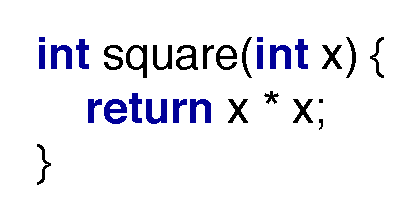
\includegraphics[width=\linewidth]{images/AstCode.pdf}
       \caption{}
       \label{fig:ast-code} 
    \end{subfigure}
    \\[\baselineskip]
    \begin{subfigure}{0.98\linewidth}
       \centering
       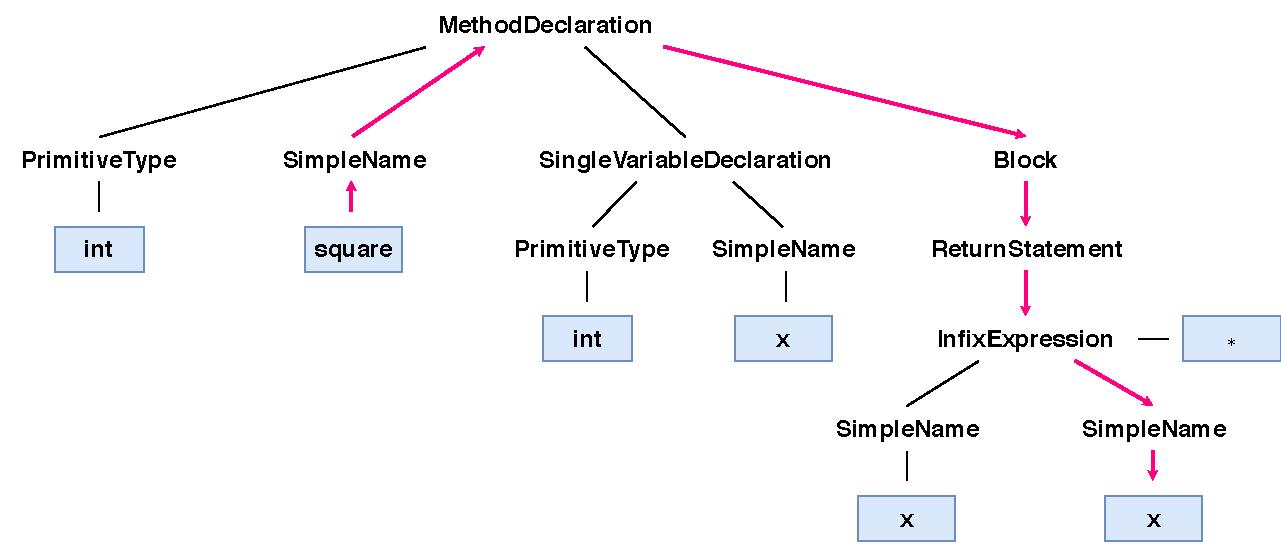
\includegraphics[width=\linewidth]{images/AstExample.pdf}
       \caption{}
       \label{fig:ast-example}
    \end{subfigure}
    \centering
    \caption{(a) Пример фрагмента кода. (b) AST, построенное по фрагменту кода при помощи библиотеки GumTree \cite{GumTree}. Цветом выделен путь между парой листьев.}
    \end{figure}

Каждому пути и токену сопоставляется вектор эмбеддинга. Эмбеддинг — это обучаемое отображение из конечного множества в векторное пространство. Изначально оно выбирается случайным, а в процессе обучения модели модифицируется. Контексту сопоставляется конкатенация из трёх векторов, соответствующих токенам и пути. Затем, чтобы получить вектор для фрагмента кода, векторизации его контекстов складываются с весами, которые им назначает механизм внимания. Он реализуется при помощи скалярного произведения вектора контекста на вектор внимания, обучаемый вместе с моделью.

В данной работе модель была дополнена путём добавления возможности работать с группами из нескольких фрагментов кода. Ими могут быть методы, относящиеся к одному коммиту или находящиеся в одном файле, случайная выборка из всего множества методов, методы, написанные в определенный промежуток времени. Для этого в неё был добавлен ещё один слой с механизмом внимания, агрегирующий векторизации нескольких фрагментов в одну. Помимо увеличения точности модели он позволяет выделить фрагменты, имеющие большее значение при решении задачи, в нашем случае — при определении авторства группы из нескольких методов. Модифицированная архитектура представлена на Рис. \ref{fig:code2vec-enhanced}.

    \begin{figure}[ht]
    \centering
       \begin{subfigure}{0.98\linewidth}
       \centering
       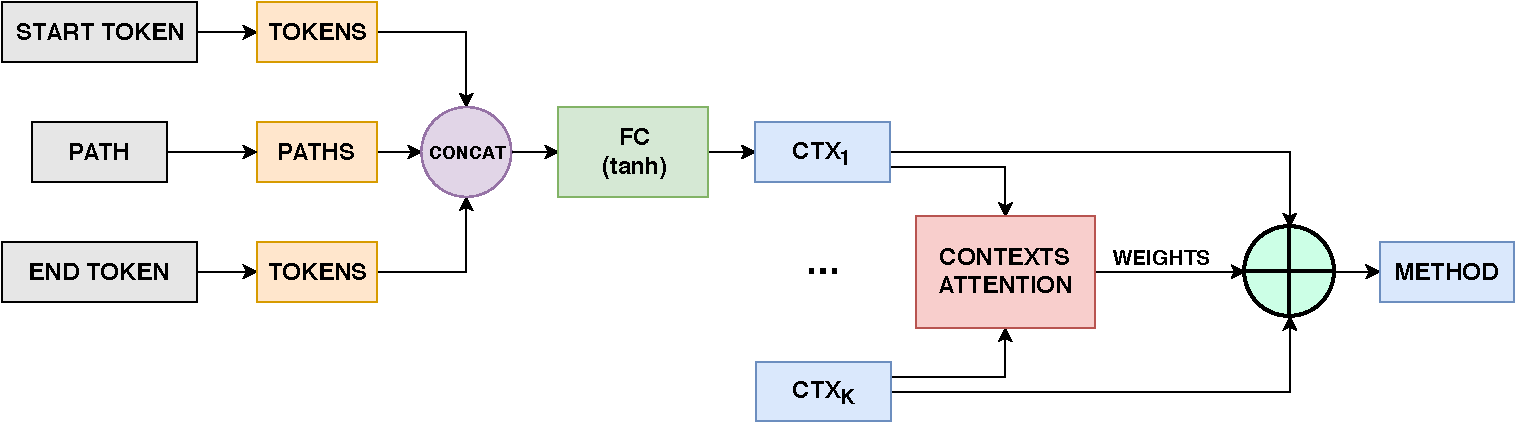
\includegraphics[width=\linewidth]{images/Code2VecOriginal.pdf}
       \caption{}
       \label{fig:code2vec-original} 
    \end{subfigure}
    \\[\baselineskip]
    \begin{subfigure}{0.34\linewidth}
       \centering
       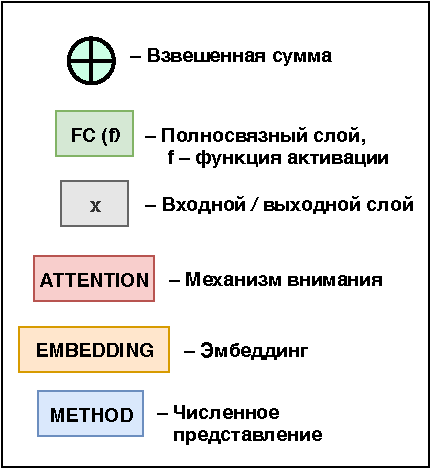
\includegraphics[width=\linewidth]{images/Code2VecLegend.pdf}
       \caption{}
       \label{fig:code2vec-legend}
    \end{subfigure}
    \hfill
    \begin{subfigure}{0.54\linewidth}
       \centering
       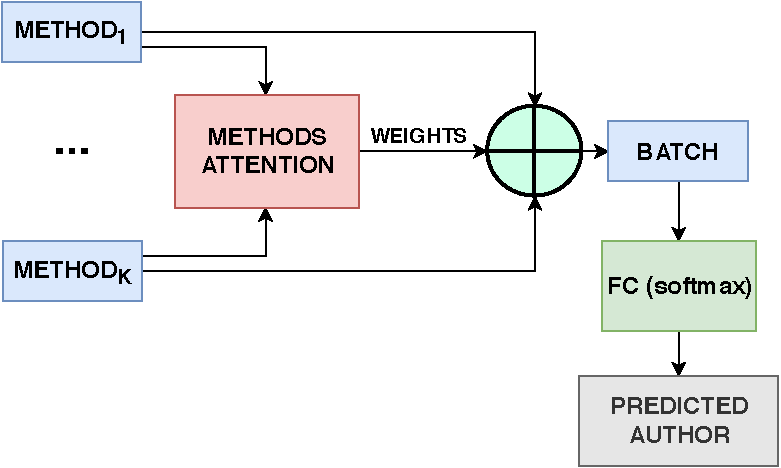
\includegraphics[width=\linewidth]{images/Code2VecEnhanced.pdf}
       \caption{}
       \label{fig:code2vec-enhanced}
    \end{subfigure}
    \centering
    \caption{(a) Архитектура модели code2vec \cite{Alon2019}. (b) Условные обозначения для описания нейросетевой архитектуры. (c) Расширение архитектуры code2vec для работы с группами из нескольких методов.}
    \end{figure}

Количество параметров в предложенной модели зависит от числа различных путей и токенов и от размерности используемых векторных представлений. Обозначим число параметров за $ModelSize$ и запишем его асимптотику:
$$ModelSize = O(Td+Pd),$$
где $T$ — число токенов, $P$ — число путей, $d$ — размерность векторизаций.

Число различных путей и токенов для датасетов, использованных в предыдущих работах, а также количество примеров, доступных для обучения, приведено в таблице \ref{tab:datasets-sizes}. Количество параметров модели даже при выборе значения размерности равного 1 остается на порядок выше, чем число примеров, поэтому для наборов данных с высоким соотношением числа различных токенов и путей к размеру датасета предлагается вторая модель.

Модель может применяться для любого языка программирования, по коду которого можно построить AST. Таковыми является большинство популярных языков программирования, так как в них AST используется компиляторами и интерпретаторами для промежуточного представления кода. Для построения AST и дальнейшего получения контекстов используется библиотека, более подробно описанная в разделе \ref{sec:data}.

\vskip 1em
	\begin{table}[ht]
      \caption{Размеры датасетов, использовавшихся в предыдущих работах и число различных токенов и путей, встречающихся в них. Приведено число различных путей с шириной не более 3 и длиной не более 10.}
		\centering
      \begin{tabular}{|c|c|c|c|}
         \hline
                                           & \textbf{C++} & \textbf{Java} & \textbf{Python} \\ \hline
         \textbf{Число авторов}            & 1600         & 40            & 70              \\ \hline
         \textbf{Размер датасета (файлов)} & 14400        & 3021          & 700             \\ \hline
         \textbf{Различные токены (тыс.)}  & 30.2         & 36.7          & 4.3             \\ \hline
         \textbf{Различные пути (тыс.)}    & 169.9        & 7.9           & 46.3            \\ \hline
         \textbf{Токены и пути / Размер}   & 13.9         & 14.8          & 72.3            \\ \hline
      \end{tabular}
		\label{tab:datasets-sizes}
   \end{table}
   
\subsection{Модель на основе случайного леса}

Вторая модель представляет из себя случайный лес. В качестве факторов используются те же данные, которые образовывали контексты, описанные выше: частоты встречаемости путей между листьями в AST и частоты встречаемости токенов на их концах. Таким образом, каждый фрагмент кода представляется разреженным вектором размера $P+2T$. Для работы модели, как и в предыдущем случае, требуется построение AST, что возможно для большинства современных языков программирования.

Для улучшения качества работы модели применяется фильтрация множества факторов при помощи подсчета совместной информации между значением фактора и автором фрагмента. Совместная информация двух случайных величин определяется следующим образом:
$$I(A;F) = H(A) + H(F) - H(A, F),$$
где $A$ — множество авторов, $F$ — множество факторов, $H(X)$, $H(Y)$, $H(X,Y)$ — энтропия и условная энтропия случайных величин.

В результате фильтрации остаются только факторы с высоким значением совместной информации с целевой функцией. Доля факторов, которая остается после фильтрации, определяется эмпирически. Полученные эмпирические значения, результаты применения модели на различных датасетах, сравнение моделей между собой и с существующими решениями приведено в главе \ref{sec:evaluation}.

У модели есть два гиперпараметра: число деревьев в лесу и количество факторов, остающихся после фильтрации. Для их подбора применяется кросс-валидация и поиск по сетке. Качество работы модели оценивается путем кросс-валидации, перебирая разные значения гиперпараметров, и эмпирически устанавливаются оптимальные значения. Они варьируются в зависимости от набора данных: оптимальная доля остающихся после фильтрации факторов составляет от 5\% до 10\%, а оптимальное число деревьев — от 300 до 500.

\subsection{Выводы}
Эта работа предлагает две модели для определения авторства в условиях разного количества данных. В обоих случаях по фрагменту кода строится AST, а затем он представляется в виде набора контекстов, состоящих из путей между парами листьев в AST и токенами на их концах. Первая из моделей — нейронная сеть, использующая механизм внимания для получения векторного представления фрагмента кода из эмбеддингов путей и токенов. Ее целесообразно использовать, когда количество различных путей и токенов сопоставимо или меньше числа доступных для обучения примеров, на практике это тысячи или десятки тысяч примеров для каждого автора. Вторая модель — случайный лес из 500 деревьев, строящийся по частотам встречаемости токенов и путей, встречающихся в фрагменте кода. Для фильтрации множества факторов применяется метод фильтрации на основании совместной информации значения фактора и автора кода. Случайный лес целесообразно использовать, когда размер датасета меньше, чем число различных путей и токенов.

\section{Тестирование}\label{sec:evaluation}
Для тестирования моделей, предложенных в главе \ref{sec:model}, применялись датасеты для трех языков, использовавшиеся в недавних работах других исследователей: решения задач GCJ для Python \cite{Alsulami2017} и C++ \cite{Caliskan2015}, набор из 40 проектов с открытым исходным кодом для Java \cite{Yang2017}. Эти три датасета представляют собой наиболее актуальные результаты для каждого из языков среди работ, использовавших данные находящиеся в открытом доступе. Результаты сравнения приведены в таблице \ref{tab:results-comparison}. Помимо тестирования на указанных датасетах были проведены эксперименты с данными проекта IntelliJ IDEA, более подробно описанными в главе \ref{sec:data}.

\subsection{Сравнение с предыдущими работами}

\subsubsection{Java}
Датасет для Java состоит из 40 проектов, написанных разными авторами. Он включает в себя 3021 файл, число файлов в проектах варьируется от 11 до 712 с медианой 54. Из-за значительного различия в числе доступных примеров между разработчиками датасет является несбалансированным. Поскольку в среднем число примеров не превышает сотни, из двух предложенных в этой работе моделей лучшие результаты показывает случайный лес, специально созданный для работы в условиях небольшого количества данных.

Сравнение производилось с лучшим на данный момент решением, использовавшим этот набор данных \cite{Yang2017}. Для получения сравнимых результатов применяется такое же разбиение данных, как и в вышеуказанной работе. Все файлы разбиваются на 10 частей, или фолдов, в каждую из которых попадает одинаковое количество примеров от каждого из авторов. Например, от разработчика с 31 файлом в одной части окажется четыре файла, а в остальных по три. Затем проводится 10 экспериментов, в каждом из которых одна часть представляет тестовую выборку, а остальные — тренировочную. По выборке, состоящей из результатов экспериментов, вычисляется выборочное среднее и дисперсия, которые затем сравниваются с результатами предыдущей работы.

Для применения случайного леса требуется подобрать оптимальные гиперпараметры, к которым относится число деревьев и количество используемых факторов. Для подбора оптимальных гиперпараметров была проведена серия экспериментов с разным количеством деревьев и разным количеством факторов. Средняя точность и отклонение, полученные в результате кроссвалидации, в зависимости от варьируемых параметров приведены на Рис. \ref{fig:hyper-trees} для числа деревьев и на Рис. \ref{fig:hyper-factors} для числа факторов. Точность при оптимальном выборе параметров значительно превосходит результаты предыдущей работы \cite{Yang2017}: 97\% против 91.1\%.


\begin{figure}[ht]
    \centering
       \begin{subfigure}{0.49\linewidth}
       \centering
       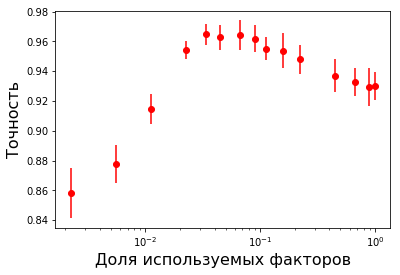
\includegraphics[width=\linewidth]{images/factors.png}
       \caption{}
       \label{fig:hyper-factors} 
    \end{subfigure}
    % \\[\baselineskip]
    \hfill
    \begin{subfigure}{0.49\linewidth}
       \centering
       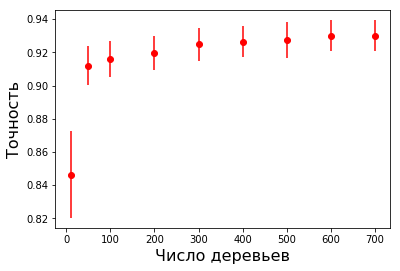
\includegraphics[width=\linewidth]{images/trees.png}
       \caption{}
       \label{fig:hyper-trees}
    \end{subfigure}
    \centering
    \caption{Зависмость точности и стандартного отклонения для датасета на языке Java от (a) доли используемых факторов; (b) числа деревьев.}
    \end{figure}

Использование нейросетевой модели показало точность 86\%, что хуже чем результаты случайного леса и нейросети, обученной при помощи PSO \cite{Yang2017}. При этом результаты оказались выше, чем у той же нейросети, обученной при помощи SGD. Это говорит о том, что даже в условиях маленького количества данных предложенная в данной работе нейросетевая модель может показывать хорошие результаты.

\subsubsection{C++}

Датасет для C++ состоит из решений задач GCJ. Он включает в себя решения по одним и тем же 9 задачам от 1600 участников. Датасет является сбалансированным, от каждого автора доступно очень мало данных, из-за чего вновь лучшие результаты показывает применение случайного леса. Для оценки качества модели используется кросс-валидация с разбиением на 9 частей, фолды представляют из себя решения по конкретной задаче. Для подбора гиперпараметров случайного леса использовался поиск по сетке.

Достигнутое значение средней точности  по итогам кросс-валидации немного меньше, чем в предыдущей работе: 92.7\% против 92.8\%. Тем не менее, стандартное отклонение результатов при кросс-валидации составляет 0.8\% и статистическая значимость различия между полученными результатами не ясна, так как авторы прошлой работы не приводят стандартного отклонения или значения точности для отдельных фолдов. Если допустить, что точность в предыдущей работе составляла 92.8\% для всех разбиений, то разница в результатах оказывается статистически незначительной.

Нейросетевая модель достигла 41.5\% точности, что значительно проигрывает случайному лесу и объясняется малым количеством доступных примеров.

\subsubsection{Python}

Датасет для Python, как и для C++, состоит из решений GCJ, но отличается размером. В нем использованы решения 10 задач от 70 участников. Для оценки точности модели применялась кросс-валидация, части разбиения состояли из пар задач. Датасет отличается от двух других еще более значительной разницей между числом доступных файлов и число различных путей и токенов (см. таблицу \ref{tab:datasets-sizes}). Из-за этого для него не удалось получить содержательной оценки работы нейросетевой модели: при точности приближающейся к 100\% на тренировочной выборке, на тестовой результаты не отличались от случайных.

Случайный лес с подобранными оптимальными параметрами показал улучшение точности по сравнению с предыдущими работами: 94\% против 88.9\%.

\vskip 1em
	\begin{table}[ht]
      \caption{Средняя точность определения авторства по итогам кросс-валидации на датасетах, использовавшихся в предыдущих работах.}
		\centering
        \begin{tabular}{|c|c|c|c|}
            \hline
                                         & \textbf{\begin{tabular}[c]{@{}c@{}}C++\\ 1600\end{tabular}} & \textbf{\begin{tabular}[c]{@{}c@{}}Python\\ 70\end{tabular}} & \textbf{\begin{tabular}[c]{@{}c@{}}Java\\ 40\end{tabular}} \\ \hline
            \textbf{Калискан и др. \cite{Caliskan2015}}            & \textbf{92.8\%}                                             & 72.9\%                                                       & -                                                          \\ \hline
            \textbf{Алсулами и др. \cite{Alsulami2017}}            & -                                                           & 88.9\%                                                      & -                                                          \\ \hline
            \textbf{Янг и др., SGD \cite{Yang2017}}            & -                                                           & -                                                            & 76\%                                                       \\ \hline
            \textbf{Янг и др., PSO \cite{Yang2017}}            & -                                                           & -                                                            & 91.1\%                                                    \\ \hline
            \textbf{Данная работа, нейросеть} & 41.5\%                                                        & -                                                            & 86\%                                                       \\ \hline
            \textbf{Данная работа, случайный лес}       & \textbf{92.7\%}                                             & \textbf{94\%}                                                & \textbf{97\%}                                              \\ \hline
            \end{tabular}
		\label{tab:results-comparison}
   \end{table}

\subsection{Тестирование на данных IntelliJ IDEA}

Для датасетов, описанных в главе \ref{sec:data}, производилось тестирование нейросетевой модели, результаты тестирования приведены в таблице \ref{tab:results-intellij}. Модель на основе случайного леса была создана для работы с меньшими объемами данных и при запуске на числе примеров близком к миллиону она столкнулась с проблемами из-за большого потребления памяти и времени, требуемого для обучения.

На каждом из датасетов нейросетевая модель обучалась при помощи оптимизатора Adam \cite{Adam} с шагом 0.01 на протяжении 10 эпох. Размерность векторизации после тестовых запусков была выбрана равной 8 для достижения баланса между пропускной способностью, сложностью модели и скоростью обучения. При этом пропускная способность была равна 1500 примерам в секунду при обучении и 2200 при тестировании.

Все 7 собранных датасетов в разной степени несбалансированные, из-за чего использование одной лишь точности для оценки качества оказывается недостаточным. Например, в датасете 3 95\% изменений методов принадлежат 40 из 50 разработчиков. В таком случае модель, которая полностью игнорирует 10 наименее активных разработчиков, может достигнуть точности 95\%. Чтобы учесть влияние несбалансированности, в дополнение к точности использовалась метрика $MAP$ (mean average precision, средняя по классам точность):
$$
MAP = \frac{1}{|A|}\sum\limits_{a \in A} precision_a,
$$
где $A$ — множество авторов, $precision_a$ — точность определения примеров разработчика $a$.

Значение $MAP$ в описанном выше случае опустится с 95\% до 80\%, что лучше отражает действительность. Помимо точности и $MAP$ использовалась $Acc_k$ (accuracy at $k$, точность для $k$) — доля примеров, для которых правильный ответ находится среди первых $k$ предсказанных. Например, $Acc_1$ это обычная точность.

\vskip 1em
	\begin{table}[ht]
      \caption{Результаты тестирования нейросетевой модели на датасетах IntelliJ IDEA.}
		\centering
        \begin{tabular}{|c|c|c|c|c|}
        \hline
                    & \textbf{Точность} & \textbf{Acc\textsubscript{2}} & \textbf{Acc\textsubscript{5}} & \textbf{MAP} \\ \hline
        \textbf{IDEA1} & 74.4\%            & 86.3\%          & 95.7\%          & 74.3\%       \\ \hline
        \textbf{IDEA2} & 99.7\%            & 100\%           & 100\%           & 99.7\%       \\ \hline
        \textbf{IDEA3} & 94.2\%            & 97.2\%          & 99\%            & 91.9\%       \\ \hline
        \textbf{IDEA4} & 97.8\%            & 99.3\%          & 99.8\%          & 97.4\%       \\ \hline
        \textbf{IDEA5} & 92\%              & 96.5\%          & 99.1\%          & 93\%         \\ \hline
        \textbf{IDEA6} & 87.3\%            & 93.2\%          & 97.7\%          & 85.9\%       \\ \hline
        \textbf{IDEA7} & 89.6\%            & 95.6\%          & 98.9\%          & 88.5\%       \\ \hline
        \end{tabular}
		\label{tab:results-intellij}
   \end{table}

Тестирование показало, что рабочий контекст оказывает значительное влияние на определение авторства: с увеличением разделения тренировочной и тестовой выборок в датасетах 4-6 значения всех метрик ухудшаются. При разделении выборок по времени точность также падает. Это может быть вызвано как изменением стиля кода авторов, так и сменой рабочего контекста, в котором находится разработчик, поскольку со временем он может менять область ответственности внутри проекта.

\subsection{Выводы}

Модель на основе случайного леса повторила лучшую на данный момент точность определения авторства на датасете для C++ и улучшила результаты для Java и Python. Нейросетевая модель из-за небольших размеров этих датасетов показала более низкие результаты и была протестирована на описанных в главе \ref{sec:data} данных IntelliJ IDEA. Из результатов тестирования можно заключить, что проверка моделей в условиях разбиения выборок по рабочему контексту и по времени должна быть изучена более подробно, например, создав обучающую выборку из данных в одном или нескольких проектах, а тестовую — из кода тех же авторов в других проектах.

\section*{Заключение}
Главным результатом данной работы стала модель, улучшающая точность определения авторства по коду на языках программирования C++, Java и Python по сравнению с имеющимися исследованиями в области. В отличие от предыдущих исследований, использовавших свойства конкретных языков и требовавших модификации решений для применения к другим языкам программирования, предложенное решение не нуждается в дополнительной модификации. Также в рамках данной работы были достигнуты следующие результаты:
\begin{itemize}
    \item Предложен метод для сбора примеров кода с известным автором из произвольных проектов, использовавших при разработке VCS git. Метод основывается на рассмотрении истории проекта и ее дальнейшем разбиении на изменения небольших фрагментов кода. С помощью предложенного подхода можно строить датасеты для тестирования решений в большем масштабе, чем это было возможно ранее, изучать поведение моделей при разбиении тренировочной и тестовой выборки во времени, изучать влияние контекста на точность определения автора кода.
    \item Предложенный подход к сбору данных был реализован и протестирован на Java-проекте с открытым исходным кодом IntelliJ IDEA. Из него было получено 2 миллиона изменений методов сделанных 500 разработчиками. Из полученных данных было сформировано 7 датасетов для тестирования моделей в разных условиях. Датасеты отличаются числом авторов, числом примеров, степенью несбалансированности. Также представлены датасеты, в которых тренировочная и тестовая выборки разбиты во времени и разделены по частям проекта. Подобные наборы данных до этого не существовали для промышленного кода.
    \item Созданы две модели для определения авторства по коду. Первая из них это нейросеть, использующая механизм внимания и эмбеддинги на основе путей и токенов в AST для векторизации одного или нескольких фрагментов кода. Предсказание автора делается по полученному вектору. Модель нацелена на использовании в случае большого количества данных, тысяч или десятков тысяч примеров от каждого из известных разработчиков. Такой масштаб достигается в крупных промышленных проектах. Вторая модель представляет собой случайный лес, обучаемый на частотах встречаемости путей и токенов в AST. Для уменьшения числа факторов и увеличения точности применяется филтрация на основе совместной информации значения фактора и автора. Модель применяется в случае небольшого количества данных, от десятка до нескольких сотен примеров от каждого автора. Обе модели не используют факторов, специфичных для конкретного языка и для применения требуют только построения AST.
    \item Улучшена точность определения авторства для датасетов на языках Python и Java, повторен результат для C++. При этом использовалась модель на основе случайного леса, поскольку датасеты в предыдущих исследованиях имели небольшой размер. Нейросетевая модель была протестирована на датасетах, собранных из проекта IntelliJ IDEA, представив базовый результат для будущих исследований.
\end{itemize}

Дальнейшая работа возможна в нескольких направлениях:
\begin{itemize}
    \item Применить предложенные модели к коду на других языках программирования. Помимо Java, C++ и Python в современных исследованиях было рассмотрено только определение авторства для Javascript \cite{Wisse2015}. Поскольку предложенные модели позволяют работать с произвольным языком, с их помощью можно расширить множество исследуемых языков.
    \item Собрать датасеты для определения авторства, моделирующие разные условия применения полученных решений. Например, поместить в тренировочную и тестовую выборки код одних и тех же разработчиков, но в разных проектах, собрать больше данных с выборками, разделенными по времени, сделать это для разных языков программирования.
    \item Научиться решать задачу профилирования разработчиков. Нейросетевая модель в процессе работы строит векторы для фрагментов кода. Эксперименты показывают, что по ним можно определять автора фрагмента. В задаче профилирования вместо этого требуется предсказать какие-то свойства автора. Ими могут выступать опыт работы, уровень экспертизы в отдельных областях, знание других языков. Решение задачи профилирования интересно для определения того, как вышеописанные свойства программиста влияют на код, который он пишет.
\end{itemize}


\bibliographystyle{ugost2008my}
\bibliography{diploma.bib}
\end{document}
